\documentclass[11pt]{article}

% basic packages
\usepackage[margin=1in]{geometry}
\usepackage[pdftex]{graphicx}
\usepackage{amsmath,amssymb,amsthm}
\usepackage{custom}
\usepackage{lipsum}
\usepackage{mathtools}
\DeclarePairedDelimiter{\ceil}{\lceil}{\rceil}

% page formatting
\usepackage{fancyhdr}
\pagestyle{fancy}

\renewcommand{\sectionmark}[1]{\markright{\textsf{\arabic{section}. #1}}}
\renewcommand{\subsectionmark}[1]{}
\lhead{\textbf{\thepage} \ \ \nouppercase{\rightmark}}
\chead{}
\rhead{}
\lfoot{}
\cfoot{}
\rfoot{}
\setlength{\headheight}{14pt}

\linespread{1.03} % give a little extra room
\setlength{\parindent}{0.2in} % reduce paragraph indent a bit
\setcounter{secnumdepth}{2} % no numbered subsubsections
\setcounter{tocdepth}{2} % no subsubsections in ToC

\theoremstyle{plain}

\graphicspath{ {./images/} }

\begin{document}

% make title page
\thispagestyle{empty}
\bigskip \
\vspace{0.1cm}

\begin{center}
{\fontsize{20}{20} \selectfont \bf \sffamily Numerical Methods for Vector Calculus}
\vskip 14pt
{\fontsize{14}{14} \selectfont \rmfamily Ian Hollas - Honors Vector Calculus - Final Project} 
\vskip 6pt
\vskip 24pt
\end{center}

\large
I implemented several numerical algorithms for solving problems involving vector calculus. Specifically, I built a program to approximate derivatives using first differences. I used this to implement gradient descent, an algorithm for finding local minima numerically. I also coded three numerical integration techniques (Monte Carlo, trapezoids, and Clenshaw-Curtis) and built a program to approximate path integrals with them. The idea was to build a ``toolbox" of programs to use in tandem with analytical techniques to produce numerical solution to vector calculus problems.
\par
The code (written in Python) can be found in a GitHub repository here: \\ https://github.com/imhollas/vector-calc. I opted to implement as much of the math myself as possible, as opposed to using external libraries. This report describes the theory behind the algorithms, how I implemented them, and their performance.


% make table of contents
\newpage
\microtoc
\newpage

% main content
\section{Finite Differences}
\indent Given a smooth function $f:\mathbf{R}\to\mathbf{R}$, we wish to efficiently approximate its derivative at a point $x_0$. The first solution one thinks of is to use the definition of the derivative,
\begin{equation*}
	f'(x_0) = \lim_{\Delta x\to 0}\frac{f(x_0+\Delta x) - f(x_0)}{\Delta x},
\end{equation*}
which naturally implies the approximation
\begin{equation*}
	f'(x_0) \approx \frac{f(x_0+\Delta x) - f(x_0)}{\Delta x}.
\end{equation*}
How good is this? We can use a Taylor series to find how the error grows with $\Delta x$:
\begin{align*}
	\epsilon &= \frac{f(x_0+\Delta x) - f(x_0)}{\Delta x} -f'(x_0)\\
	&= \frac{f'(x_0)\Delta x + f''(x_0)\Delta x^2/2 + O(\Delta x^3)}{\Delta x} - f'(x_0) \\
	&= f''(x_0)\Delta x /2 + O(\Delta x^2).
\end{align*}
So the error for this approximation is linear with the step size. Surprisingly, we can do better for free by taking a ``centered difference" instead of a ``forward difference":
\begin{equation*}
	f'(x_0) \approx \frac{f(x_0+\Delta x) - f(x_0-\Delta x)}{2\Delta x}.
\end{equation*}
The $f''$ terms in cancel, so the error is quadratic in the step size:
\begin{align*}
	\epsilon &= \frac{f(x_0+\Delta x) - f(x_0-\Delta x)}{2\Delta x} - f'(x_0) \\
	&= \frac{[f''(x_0)(\Delta x)^2/2 + O(\Delta x^3)] - [f''(x_0)(-\Delta x)^2/2 + O(\Delta x^3)]}{2\Delta x} \\
	&= O(\Delta x^2).
\end{align*}
\indent I used this idea (which I found in Strang, see sources) in my program (gradient.py) that numerically evaluates the gradient of any function at a given point. The program takes a function, a position, and a step size and outputs the vector of partial derivatives. One could easily apply use this to compute other things of interest (Jacobian, divergence, curl). The gradient, in particular, has an interesting application to minimization problems, as discussed in the next section. 
\par
\textbf{Sidenote on notation:} Above we used big-O notation to refer to the leading term in a Taylor series. Everywhere else in this document, it is used to refer to the time complexity of a program, following the conventions used in computer science: $O(f(N))$ means that as $N\to\infty$ (where $N$ is the size of the input), the dominant term in the growth in the number of elementary operations is $f(N)$.
\par
How does our implementation actually perform? We use $f(x)=e^x$ at $x=0$ as a test case. The time complexity is $O(1)$, with respect to $\Delta x$ as the input; we dont expect smaller $\Delta x$ to be more computationally expensive. Experimentally, testing computing time for smaller $\Delta x$ suggests little to no correlation between the two up to $\Delta x = 10^{-13}$: \\
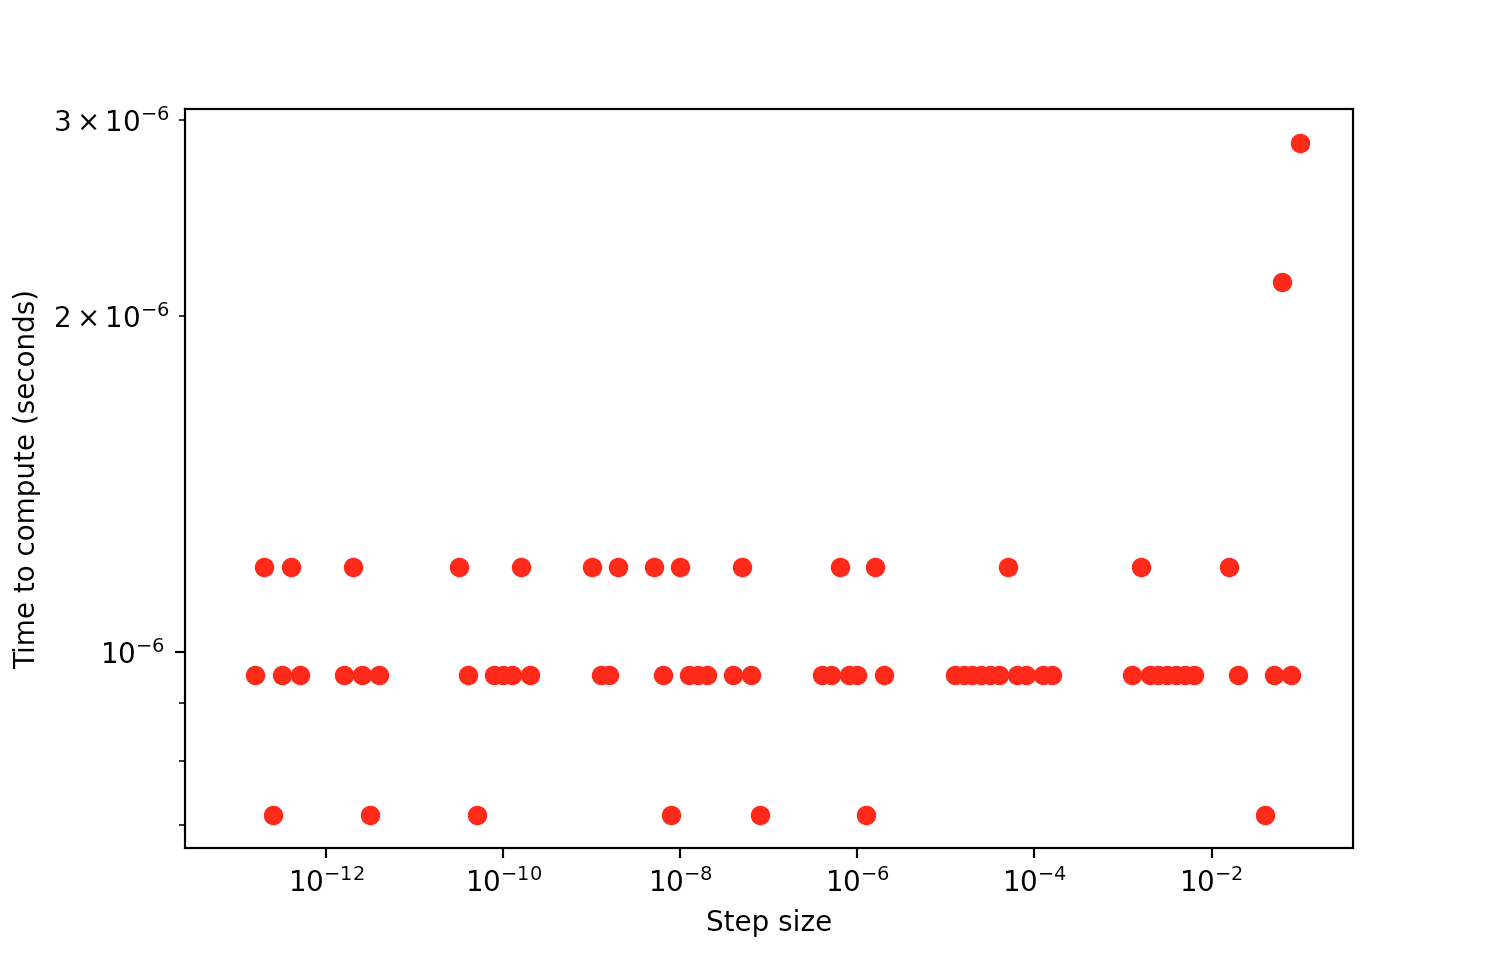
\includegraphics[scale=0.5]{finitedifftime}
\\ But there ought to be some kind of limit to our accuracy. We test the error in the algorithm with decreasing step size to find out where: \\
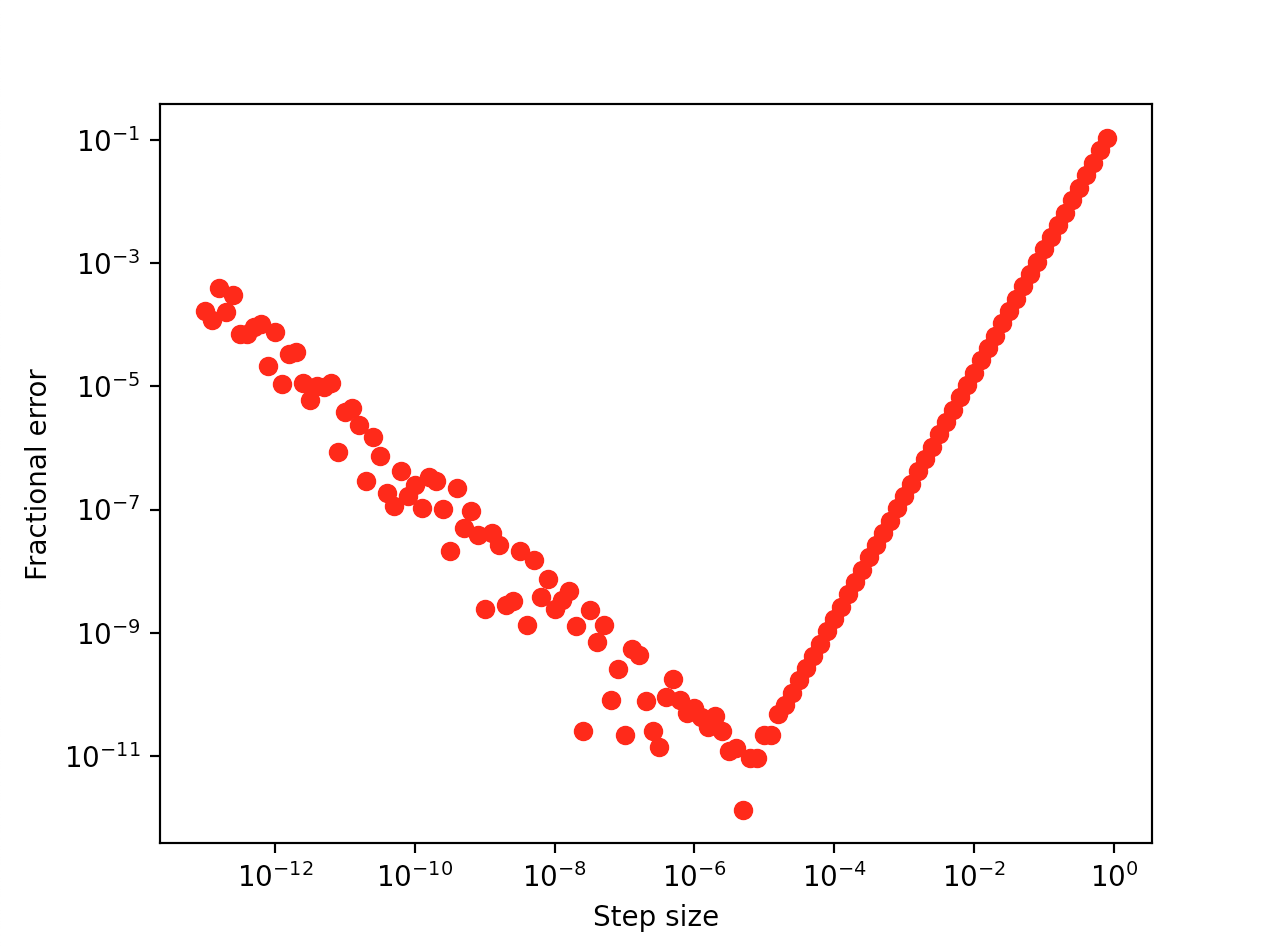
\includegraphics[scale=0.5]{finitediff}
\\ Note that the scales are logarithmic and step size decreases as you go left. Up to a step size of $\sim 10^{-5}$, it seems to follow a quadratic, after which point the data becomes rougher and the error increases. As there's no mathematical reason for the error to increase like this, this is most likely due to how the computer deals with very small numbers (floating point error). 

\section{Gradient Descent}
A common problem in vector calculus is to find the extrema of a function. State concretely, given a smooth function $f:D\to\mathbf{R}$ with $D\subseteq\mathbf{R}^n$, we wish to find local minima (or maxima) of $f$ on $D$. To do this numerically, I implemented a basic version of an algorithm called gradient descent. The idea is to start at a random point in $D$, compute the gradient $\nabla f$ at that point (analytically or numerically), and then take a step $\alpha \nabla f$, where $\alpha$ is a constant. For minima, choose $\alpha<0$, and for maxima, choose $\alpha>0$. This process is repeated until $|\nabla f|<\epsilon$ for some small $\epsilon$ (my code uses $\epsilon = 10^{-5}$), or $N\gg1$ steps occur (to ensure the program terminates; I used $N=10^7$). The program returns the current position and the number of steps taken. \\
\indent For code testing, I used problem 3 from homework 4: minimize $f(x,y) = xy + 1/x + 1/y$ on the first quadrant. I restricted to $D = (0,100)\times(0,100)$ since I need a bounded domain to choose a random point. Analytically, we can show that this function has a local minima at $(1,1)$. I ran 1000 trials of choosing a random point in the domain and running the algorithm described above with $\alpha = -1$. The gradient was computed numerically using the approximation from the previous section. The process ended outside of $D$ 624 times, so we ignore those cases. It converged to $(1,1)$ in the other 376 trials, on average within $5\cdot10^{-5}$. It took an average of $\sim 8900$ steps, with standard deviation $\sim 3600$. 
\par
\indent While they weren't necessary for this particular problem, some possible optimizations include decreasing $|\alpha|$ as the number of steps increases (so that we jump around a lot less as we get closer to the target), stopping if we leave $D$ instead of continuing to try and find extrema (since we only care about extrema in $D$), and finding the gradient analytically instead of approximating it (in problems where this is possible).
\section{Numerical Integration: Trapezoid Rule}
The basic problem: given a function $f:[a,b]\to\mathbf{R}$, efficiently approximate the integral $I$ of that function over the interval. Analytic techniques (setting up bounds) can be used in conjunction with the methods here to integrate functions on domains in $\mathbf{R}^n$.\\
\indent The first method that I used is the trapezoid rule. The idea is to divide the interval into $N$ even subintervals. We can approximate the integral $I_k$ over the $k$th subinterval by
\begin{equation*}
	I_k \approx \frac{f(a+(k-1)\Delta x) + f((a+k)\Delta x)}{2}\Delta x,
\end{equation*}
where $\Delta x = (b-a)/N$. Geometrically, this approximates the function by a trapezoid, hence the name. Summing for each subinterval gives
\begin{align*}
	I \approx \sum_{k=1}^N \frac{f(a+(k-1)\Delta x) + f((a+k)\Delta x)}{2}\Delta x \\
	= \Delta x\left[\frac{f(a)+f(b)}{2} + \sum_{k=1}^{N-1} f(a + k\Delta x)\right].
\end{align*}
One can prove this converges for continuous $f$ by using the intermediate value theorem to show that the sum above is a Riemann sum relative to the partition of $[a,b]$ into $N$ even subintervals, so the sum converges to $I$ as $N\to\infty$.
\par
An analysis of the error in the trapezoid rule can be found in Johnson (see sources). In short, since the trapezoid rule apprxoimates the function locally by its derivative, the error in the function on a single subinterval is proportional to $\Delta x^2$, so the error in the area per subinterval is proportional to $\Delta x^3 \propto 1/N^3$. There are $N$ subintervals, so the error is worst-case proportional to $1/N^2$. This is worst-case because it assumes that the errors in the subintervals always add and don't cancel, which they tend to for periodic functions. The method in the next section exploits this.
\par
\indent My implementation (trapezoid.py) directly implements the sum above using a for-loop. As this takes $N+1$ functions calls, the time complexity of the program is $O(N)$.
\section{Numerical Integration: Clenshaw-Curtis}
A technique called Clenshaw-Curtis quadrature uses change of variables to get exponential convergence with the trapezoid rule (for smooth functions). My theoretical explanation is heavily based on Johnson (see sources section), from which I learned this.
\par 
Without loss of generality, we wish to approximate $I=\int_{-1}^1 f(x)\, dx$ (my implementation begins by changing variables to this). We make a change of variables $x=\cos \theta$, so $I=\int_0^\pi f(\cos\theta)\sin\theta \, d\theta$. Note that $f(\cos\theta)$ is even and periodic on the bounds. We then expand $f(\cos\theta)$ as a Fourier series and evaluate analytically,
\begin{equation*}
	f(\cos\theta)=\frac{a_0}{2}+\sum_{k=1}^\infty a_k\cos(k\theta),
\end{equation*}
so the integral becomes
\begin{align*}
	I &= \int_0^\pi \left[\frac{a_0}{2}+\sum_{k=1}^\infty a_k\cos(k\theta) \right]\sin\theta \, d\theta\\
	&= a_0 + \sum_{k=1}^\infty a_k \int_0^\pi \cos(k\theta)\sin\theta\,d\theta \\
	&= a_0 + \sum_{k=1}^\infty a_k \frac{\cos(\pi k)+1}{1-k^2} \\
	&= a_0 + \sum_{k=1}^\infty \frac{2a_{2k}+1}{1-(2k)^2}.
\end{align*}
The coefficients are found by calculating
\begin{equation*}
	\frac{2}{\pi}\int_0^\pi f(\cos\theta)\cos(k\theta)\,d\theta
\end{equation*}
via the trapezoid rule. This seems worse at first, since now we have to compute a bunch of trapezoid sums. But, because $f(\cos\theta)\cos(k\theta)$ is periodic on the bounds, the errors in the sums tend to cancel, so the trapezoid sums converge exponentially fast. Additionally, since $f(\cos\theta)$ was constructed to be even around $0$ and $\pi$, its Fourier series converges quickly as well, so we don't need that many terms. My code only computes up to $a_N$ (only $N/2+1$ coefficients).
\par
My program first defines a new function $g$ such that $\int_{-1}^1 g(x)\,dx = \int_a^b f(x)\,dx$ ($f$ refers to the function we wish to integrate). In order to compute each trapezoid sum for $a_k$, we will need $g(\cos(n\pi/N))$ for $n=0$ through $n=N$. There's no point in computing them again for each coefficient, so it computes them all at once and stores them in a list. Then my code uses this to compute the coefficients, sums them as above, and returns the value. Since we still have to do around $N$ function calls for each of the $N/2$ coefficients, the time complexity of the program is $O(N^2)$. This is worse than the trapezoid rule (which, recall, is $O(N)$), but, as we'll see, the speedier convergence more than makes up for this.
\section{Numerical Integration: Monte Carlo}
The last technique I implemented is a version of the Monte Carlo technique. The basic idea is to pick a random point $t_i\in[a,b]$, evaluate $f(t_i)$, repeat this $N \gg 1$ times, and average to get
\begin{equation*}
	I \approx \frac{b-a}{N} \sum_{i=1}^N f(t_i).
\end{equation*}
The point choosing process can be described by a probability distribution function $p:[a,b]\to \mathbf{R}$ defined by $p(x) = 1/(b-a)$. The expected value of $f(x)$ is therefore 
\begin{align*}
	\langle f(x)\rangle &= \int_a^b f(x) p(x)\, dx = \frac{1}{b-a}\int_a^b f(x)\, dx = \frac{I}{b-a}.
\end{align*}
By the law of large numbers, the random process of choosing $t_i$, evaluating $f$, and averaging will converge to $\langle f(x)\rangle$ as $N\to\infty$, so this method does approximate $I$. \\
\indent My program uses a function from a Python library to generate a random number in $[a,b]$, calls the function being integrated, repeats $N$ times, and averages the result. The time complexity is $O(N)$, since we do a set number of operations for each repetition.
\section{Numerical Integration: Data and Comparisons}
I tested programs on the integral
\begin{equation*}
	\int_0^1 e^x + 1 \, dx = e.
\end{equation*}
Below is the result for the trapezoid rule (note that the axes are logarithmic): \\
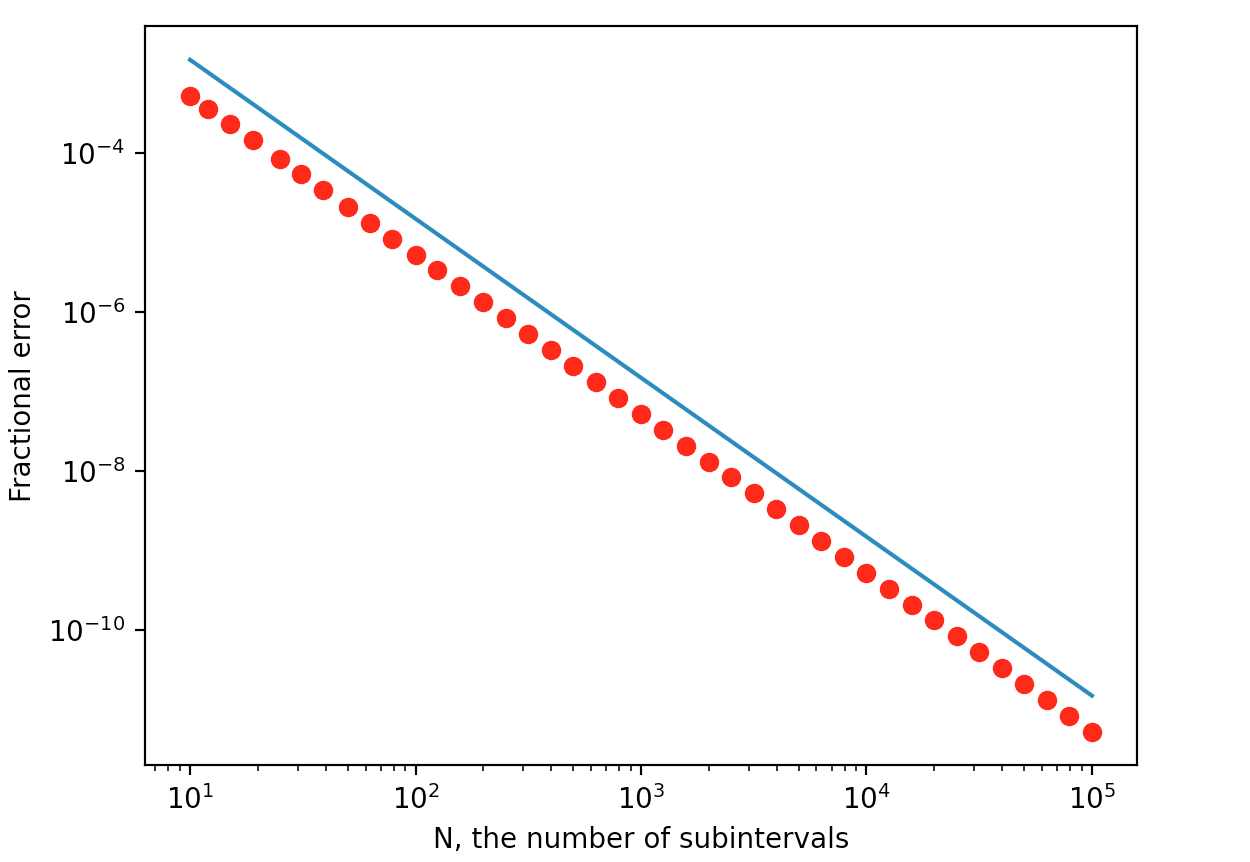
\includegraphics[scale=0.5]{trapezoiddata}
\\ The red dots are data points, the blue line is the graph of $y = a/x^2$ (with $a$ constant). We see that the error in my program agrees with theory: it roughly decreases with $1/N^2$. How much better does my implementation of Clenshaw-Curtis quadrature do on the same problem? \\
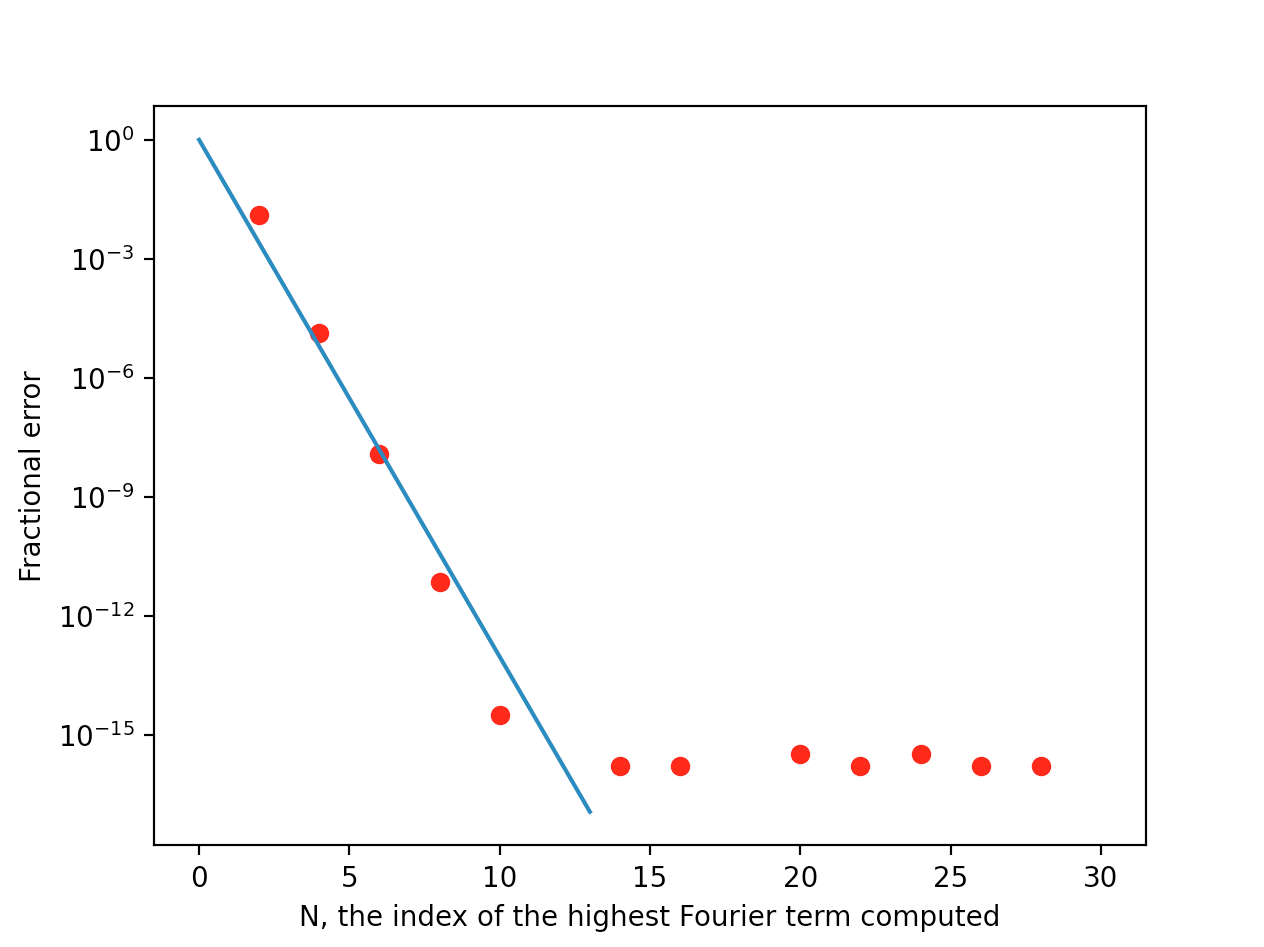
\includegraphics[scale=0.5]{ccdata}
\\ Note that the scale on the $x$-axis is linear, instead of logarithmic. The blue line is the graph of $y = e^{-3x}$. We see that the error drops way faster than the trapezoid rule! It gets more accuracy computing up to $a_{10}$ than the trapezoid does with $10^5$ subintervals! This more than makes up for the program being $O(N^2)$ instead of $O(N)$; we need comparatively such a small $N$ that it doesn't matter! Interestingly, the error bottoms out at $\sim10^{-15}$. My best guess is that on that order of magnitude, floating point error (error due to the computer only representing some numbers and approximating the rest) accumulates and causes the accuracy to ``bottom out" like it does above. Lastly is the Monte Carlo method: \\
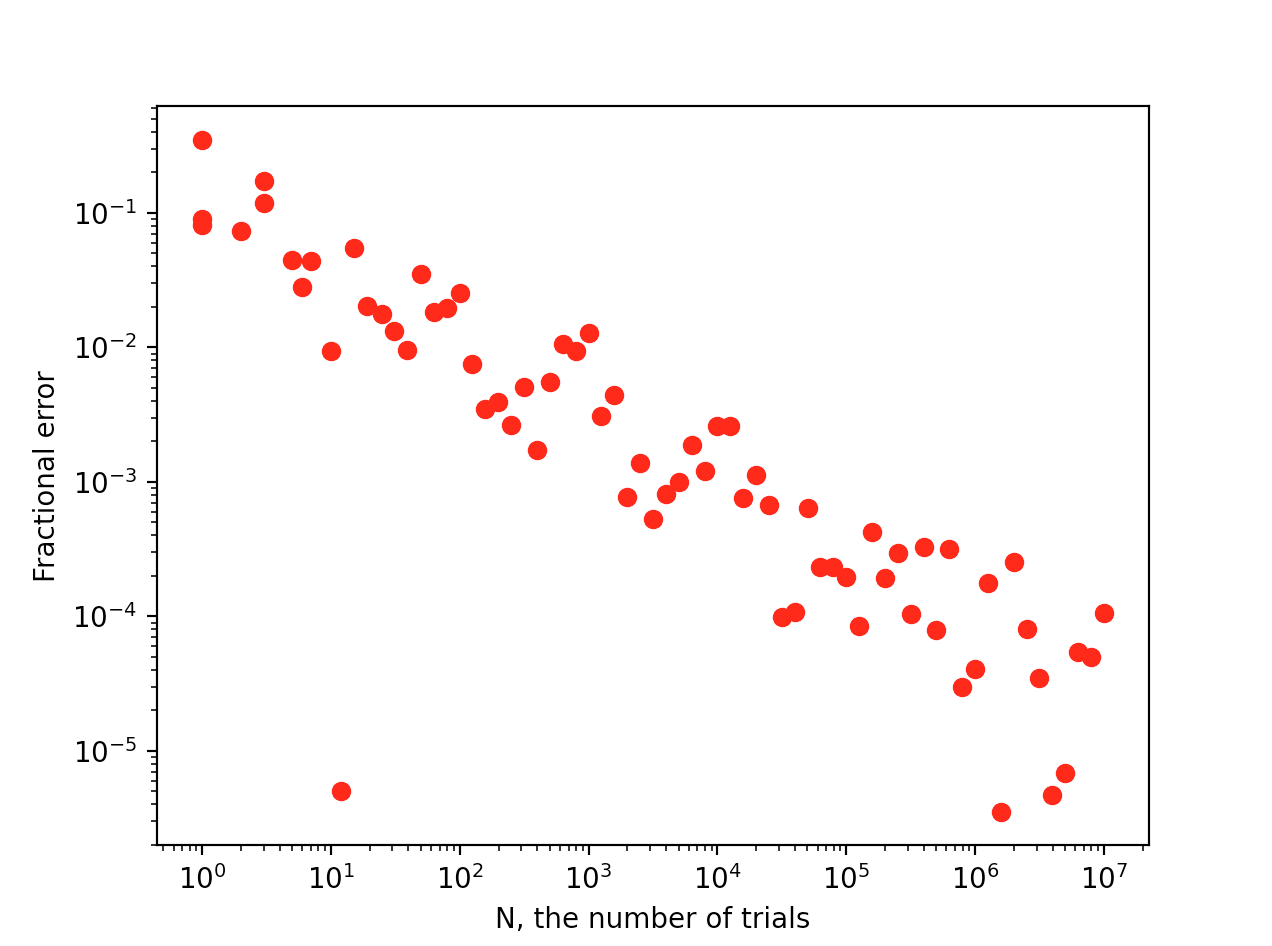
\includegraphics[scale=0.5]{montecarlo}
\\ It definitely converges slower than both Clenshaw-Curtis and the trapezoid rule, taking $10^7$ trials to get the kind of accuracy that takes the trapezoid rule around $100$ subintervals. 
\par 
It's important to note, however, that our test function is rather well behaved, being not only continuous but infinitely differentiable. Clenshaw-Curtis and the trapezoid rule both rely on the function being at least somewhat ``nice." For example, if the function is discontinuous in some places, than the trapezoid sums are not necessarily Riemann sums, in which case the proof mentioned for its convergence fails. Based on my data, then, Monte Carlo seems like it would be most useful for integrating functions whose ``niceness" is unknown. Assuming the function is continuous and smooth, my implementation of Clenshaw-Curtis is clearly preferred. But if I wanted to numerically integrate, say, the Weierstrass function, I'd start with Monte Carlo.
\section{Line Integrals}
As an application of the work in the previous section, I wrote a program (lineintegrals.py) that uses a numerical integration program (compatible with any of the ones I wrote and discussed) to compute line integrals. The vector operations are implemented by representing vectors as lists in Python. For example, a vector field in $\mathbf{R}^3$ is built by writing a function that takes in a list (representing coordinates) and returns a list (representing the vector value of the field at that point). Paths are represented parametrically and the velocity vector is found using the finite difference techniques discussed previously. The program then creates a function approximating the integrand (taking the dot product) and passes it to a numerical integration program to compute the line integral.
\par
As a test case, I used problem 8 from problem set 8, integrating $\mathbf{F}(x,y) = -y^3\mathbf{i}+x^3\mathbf{j}$ around the unit circle. The theoretical value is $3\pi/2$. Using a finite difference step size of $10^{-4}$ and computing up to the 20th term in the Clenshaw-Curtis sum, the program got it within $\sim 4\cdot10^{-6}$ with a runtime of $\sim 55$ microseconds.
\section{Sources}
\begin{enumerate}
	\item \emph{Computational Science and Engineering}. Strang, Gilbert. 2007.
	\item \emph{Numerical integration and the redemption of the trapezoid rule}. Johnson, S. G. 2011. MIT Applied Math, IAP Math Lecture Series 2011. https://ocw.mit.edu/courses/18-335j-introduction-to-numerical-methods-spring-2019/resources/mit18\_335js19\_lec33\_1/
	\item \emph{Gradient descent, how neural networks learn}. Sanderson, Grant (3Blue1Brown). 2017. https://www.youtube.com/watch?v=IHZwWFHWa-w
\end{enumerate}
The centered difference trick in section 1 I learned from Strang. The trapezoid rule I remembered vaguely from my calculus course and derived it from there. I found out about Clenshaw-Curtis quadrature in Johnson after searching for improvements on the trapezoid rule. The theoretical convergence rate of the trapezoid rule is from there. I heard about gradient descent in Sanderson's video.
\end{document}
